\begin{comment}
\begin{itemize}
    \item How to enable the Analytics service~\url{https://developer.huawei.com/consumer/en/doc/development/HMSCore-Guides-V5/service-enabling-0000001050745155-V5} and see \url{https://developer.huawei.com/consumer/en/codelabsPortal/carddetails/HMSAnalyticsKit}. There's also a codelab for enabling analytics in Kotlin~\url{https://developer.huawei.com/consumer/en/codelabsPortal/carddetails/HMSAnalyticsKit-Kotlin}. There's also the article on Medium~\sidecite{huawei2020_appgallery_connect_crash_service_article_on_medium} and the associated source code on GitHub~\url{https://github.com/SerkanMUTLU/Huawei-AppGallery-Crash-Service}.
    \item How the Crash Service works \url{https://developer.huawei.com/consumer/en/doc/development/AppGallery-connect-Guides/agc-crash-introduction-0000001055732708}. Three steps: 1) integrate the SDKs, 2) test the crash service, and 3) analyse a crash. 
    \item Their Android Sample Code is available \url{https://developer.huawei.com/consumer/en/doc/development/HMSCore-Examples/android-sample-code-0000001050745043}
    \item Pre-release Check for their Analytics SDK \url{https://developer.huawei.com/consumer/en/doc/development/HMSCore-Guides-V5/android-pre-release-check-0000001050420841-V5}, which includes a spreadsheet (which I've downloaded) that covers basic sanity testing.
    \item Lots of clear articles (still lacking in various details) that help to understand how their analytics SDK behaves and how that behaviour can be modified (and checked) by developers. For example~\sidecite{huawei_accessing_analytics_kit}.
    \item Online training videos on their Analytics software \url{https://developer.huawei.com/consumer/en/training/detail/101582991973534154}
    \item Cloud Testing articles \href{https://forums.developer.huawei.com/forumPortal/en/topic/0201271583209350068}{Part 1} and \href{}{Part 2}. And a more structured article~\url{https://developer.huawei.com/consumer/en/doc/development/AppGallery-connect-Guides/agc-cloudtest-introduction-0000001083002880}.
    \item Developer reports he cannot see crashes for the productFlavor that should use the Huawei crash reporting~\url{https://stackoverflow.com/questions/64800108/can-not-see-crashes-for-android-on-appgallery-connect}. It's not clear whether a) the library needs to be instantiated by the application at runtime, b) if there'll be conflicts between the Huawei and Google Firebase crashlytics libraries and/or instantiation.
    \item \url{https://developer.huawei.com/consumer/en/appgallery/} marketing to the developers.
    \item \url{https://developer.huawei.com/consumer/en/codelabsPortal/index} HUAWEI Codelabs.
    \item \url{https://stackoverflow.com/questions/tagged/huawei-mobile-services} Active support from Huawei for developers.
    \item \url{https://stackoverflow.com/questions/67885601/react-native-app-crashes-while-launching-after-implementing-hmscore} Interesting answer from Shirley who works for Huawei I believe about how their support HMS Core on non-Huawei devices \url{https://stackoverflow.com/a/67886284/340175} - Details saved in my references in the HUAWEI folder.
    \item App Rollbacks \textit{are} supported! \url{https://developer.huawei.com/consumer/en/doc/distribution/app/agc-help-rollback-0000001146534647}
    \item Developers can provide messages in the app store for their users \url{https://developer.huawei.com/consumer/en/doc/distribution/app/agc-help-developers-message-0000001146438657}
    \item \emph{Intermediate: Easy fix of application crash using Huawei Crash Service and Remote Configuration}~\url{https://forums.developer.huawei.com/forumPortal/en/topic/0202581794223780039}
\end{itemize}
\end{comment}



\begin{table*}
    \centering
    \resizebox{\textwidth}{!}{% See https://tex.stackexchange.com/a/27105/88466 TODO improve the readability of the table.
    \begin{tabular}{c|ccccc}
        \toprule
        \textit{stage} & During init & During shutdown & In background service & In `flight' & In a `runtime' \\
        \midrule
         Mobile Analytics tool & & & & & \\
         \midrule
         Google Play Console with Android Vitals & C & C & C & C & \\
         Fabric Crashlytics &  & Unknown & Unknown & EC & \\
         Sentry & N & & & Y & Y \\
         \bottomrule
    \end{tabular}}
    \caption[Mapping error and crash reporting to mobile analytics tools]{Mapping error and crash reporting to mobile analytics tools \\ E = Error, C = Crash, B = Breadcrumb, K = Custom content, N = No}
    \label{tab:discussion-mapping-error-and-crash-reporting-to-ma-tools}
\end{table*}
\afterpage{\clearpage}

TODO discuss: the reporting mechanisms and limitations in addition to Table~\ref{tab:discussion-mapping-error-and-crash-reporting-to-ma-tools}'s examples of what they can capture. Also discuss the primary focus of this research has been on Crashes, then on Errors, then on ANRs~\todo{Note: this material probably belongs in the Tools chapter once I've established it.}.


A couple of examples of poor user experiences that don't involve crashes or freezes (so would not be detected using the platform-level analytics) are, the Financial Times Android app: Figure~\ref{fig:ft_android_app_bsod}, and The Times newspaper iOS app: ``Cannot find article: Apologies, this article no longer exists." Figure~\ref{fig:thetimes-ios-this-article-no-longer-exists}. Of these, the missing article could be recorded easily using in-app error reporting (it might be detected by a non-fatal exception using a crash-reporting library or mobile analytics). The black screen is likely to be harder to report on (as if the developers were aware of the potential for the problem they could add error-handling and error-recovery logic).

\begin{figure}[!htbp]
    \centering
    \subfloat[What the user sees] {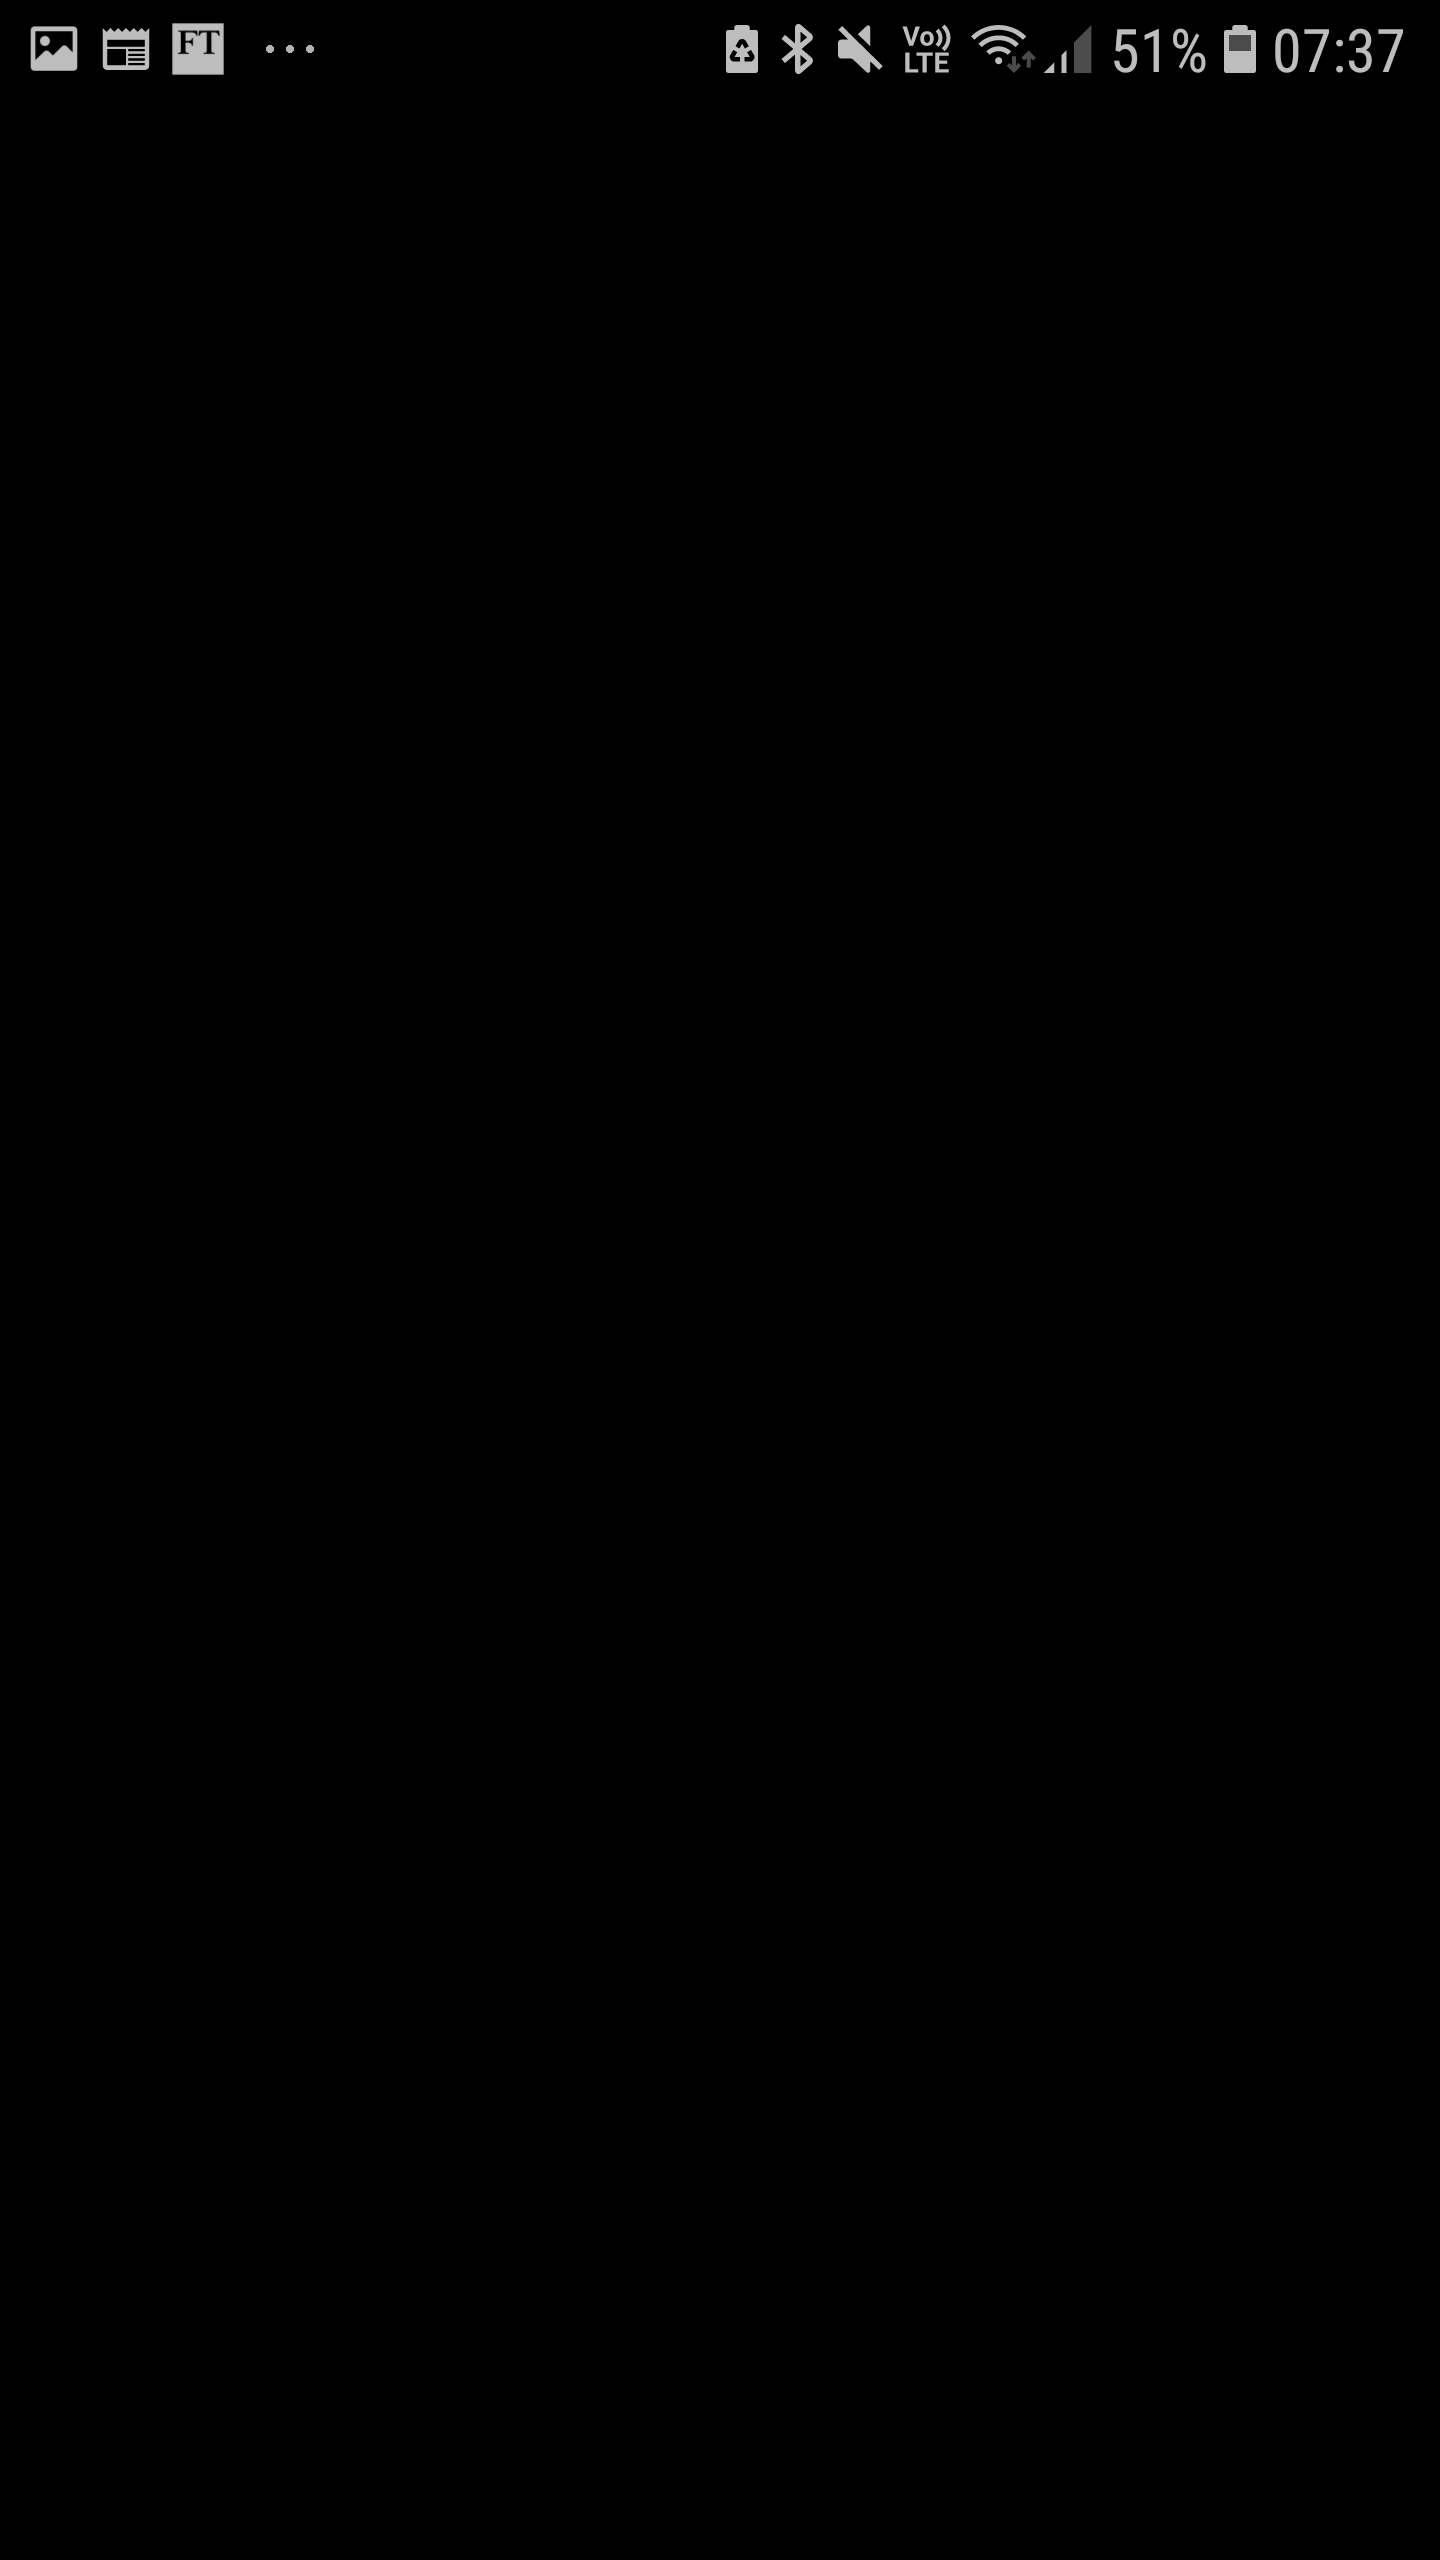
\includegraphics[width=0.45\textwidth]{images/android-screenshots/Screenshot_20200928-073727_FT.jpg}\label{fig:android_ft_GUI}}
    \hfill
    \subfloat[The FT app in the task list] {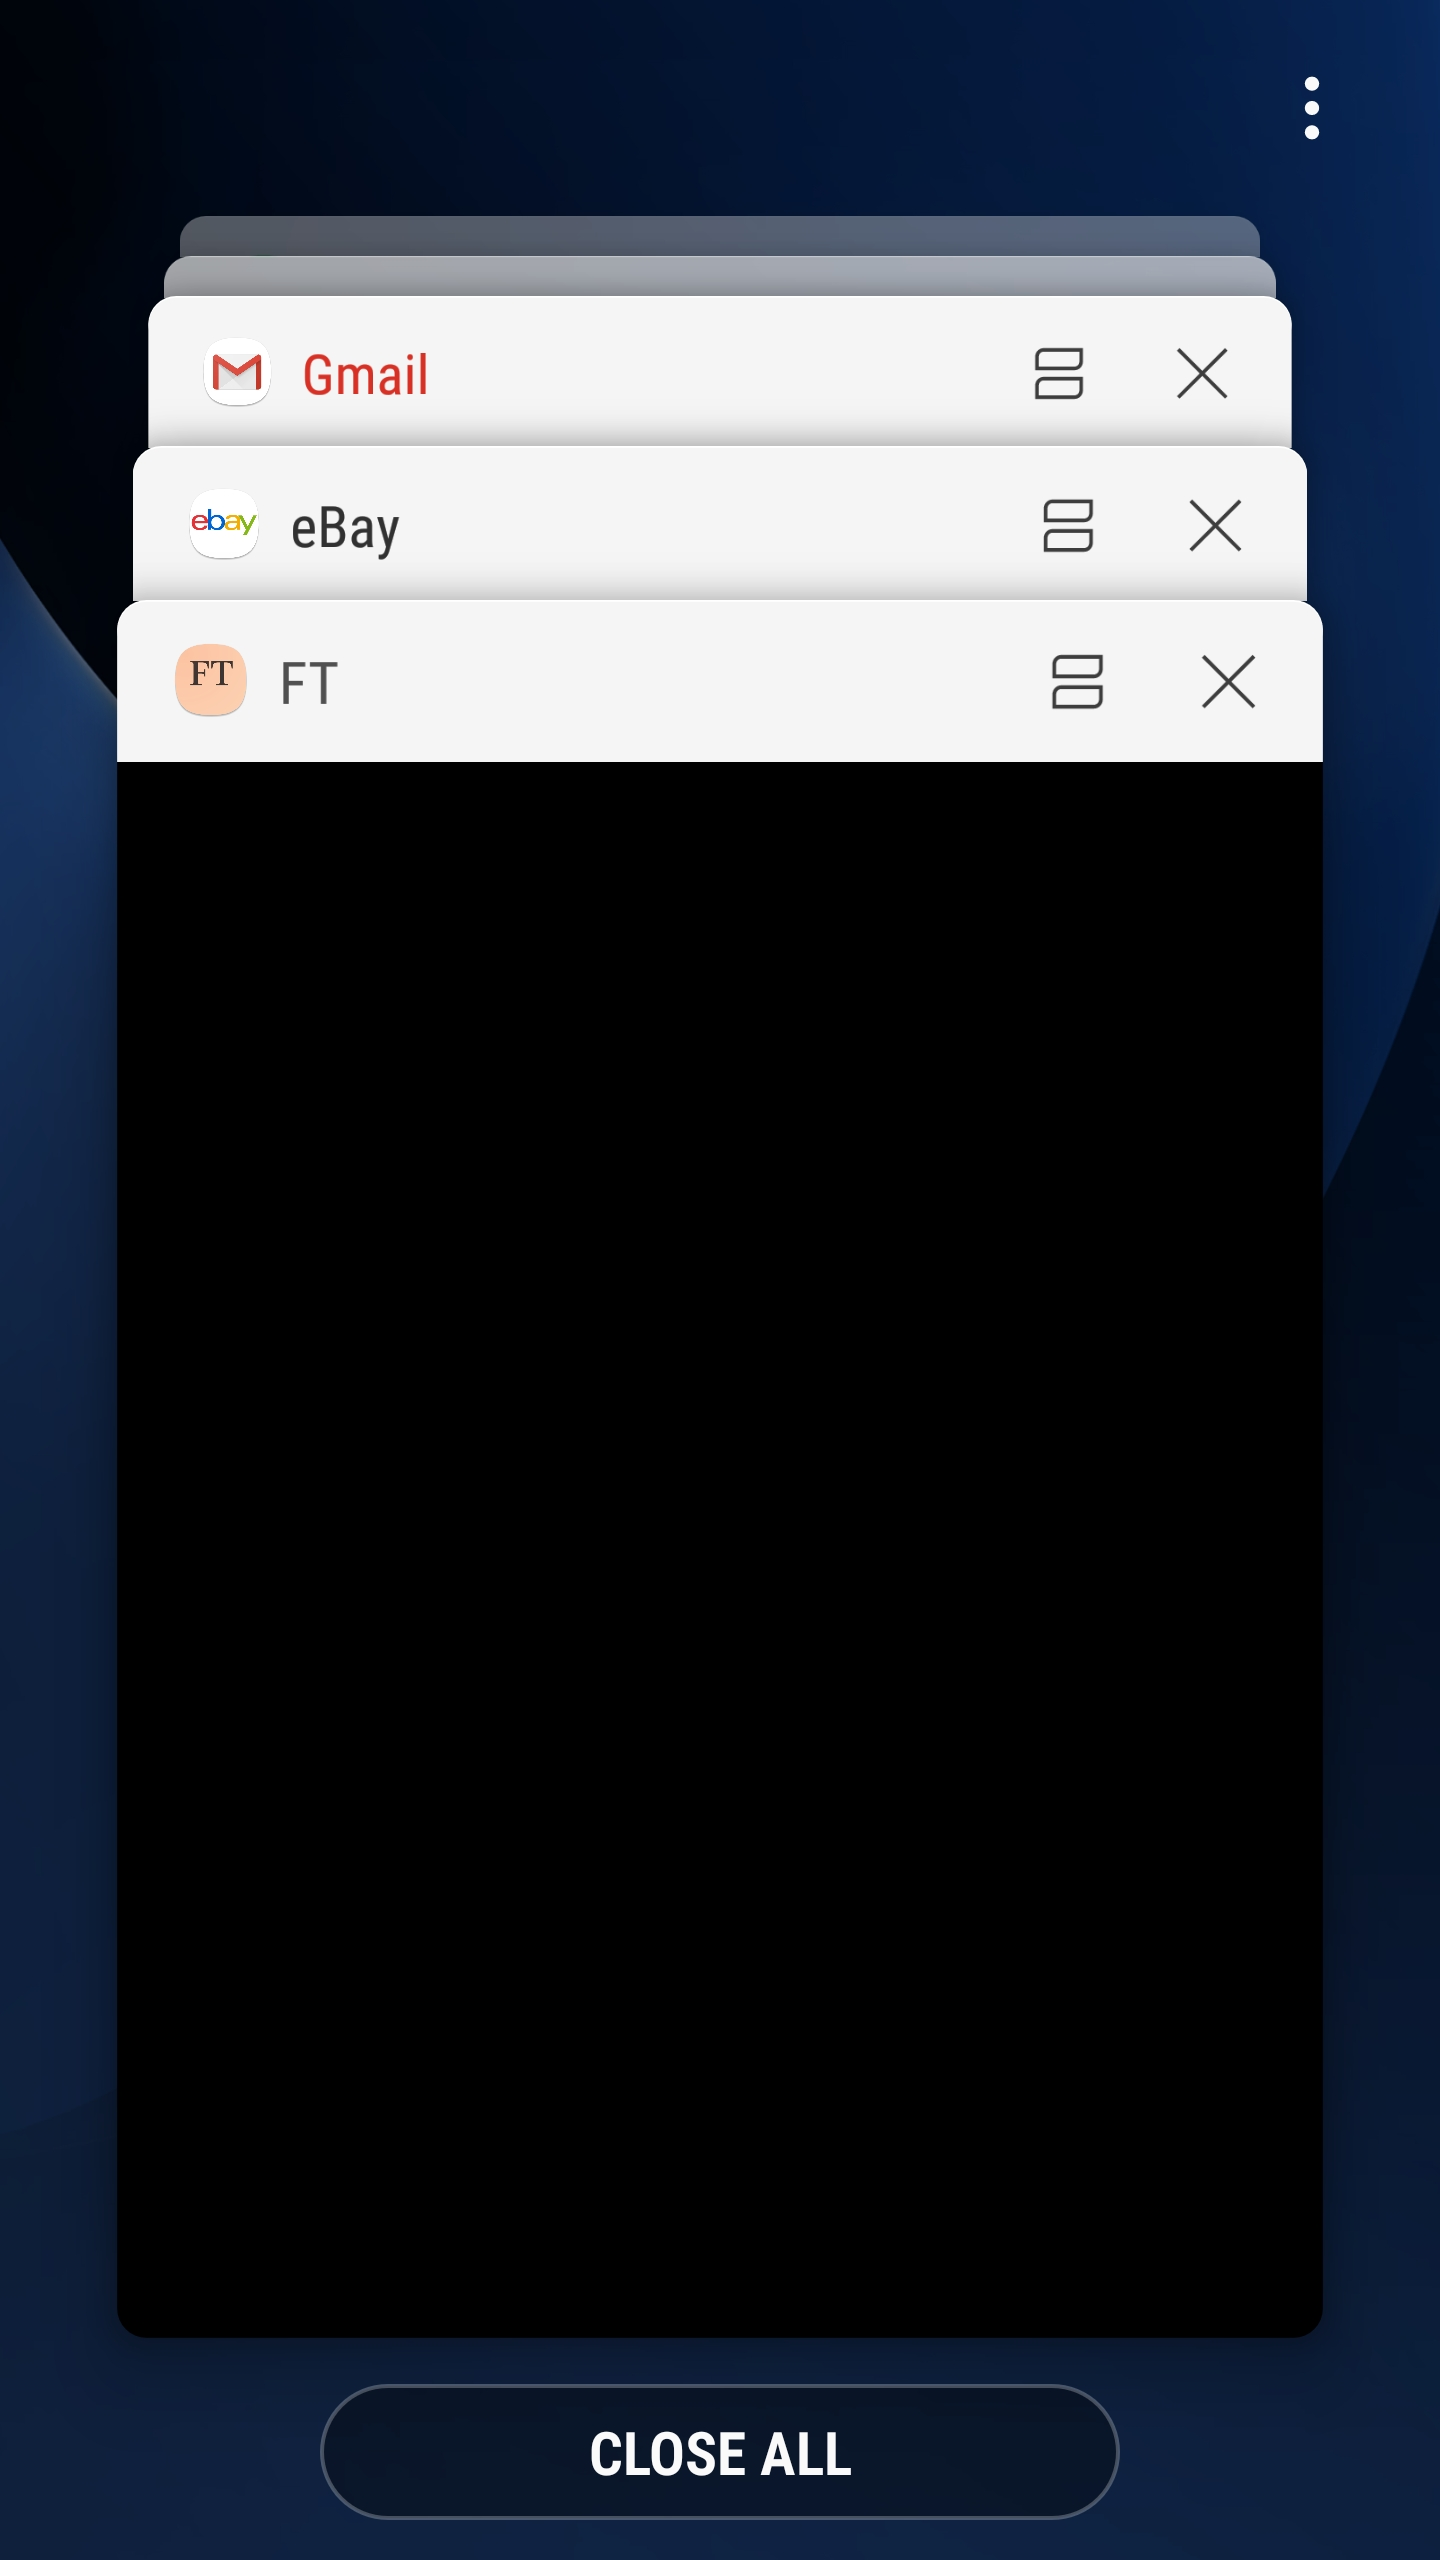
\includegraphics[width=0.45\textwidth]{images/android-screenshots/Screenshot_20200928-073745_FT.jpg}\label{fig:ft_android_app_in_task_list}}
      \caption{Black screen when notification selected}
    \label{fig:ft_android_app_bsod}
\end{figure}

\begin{figure}[!htbp]
    \centering
    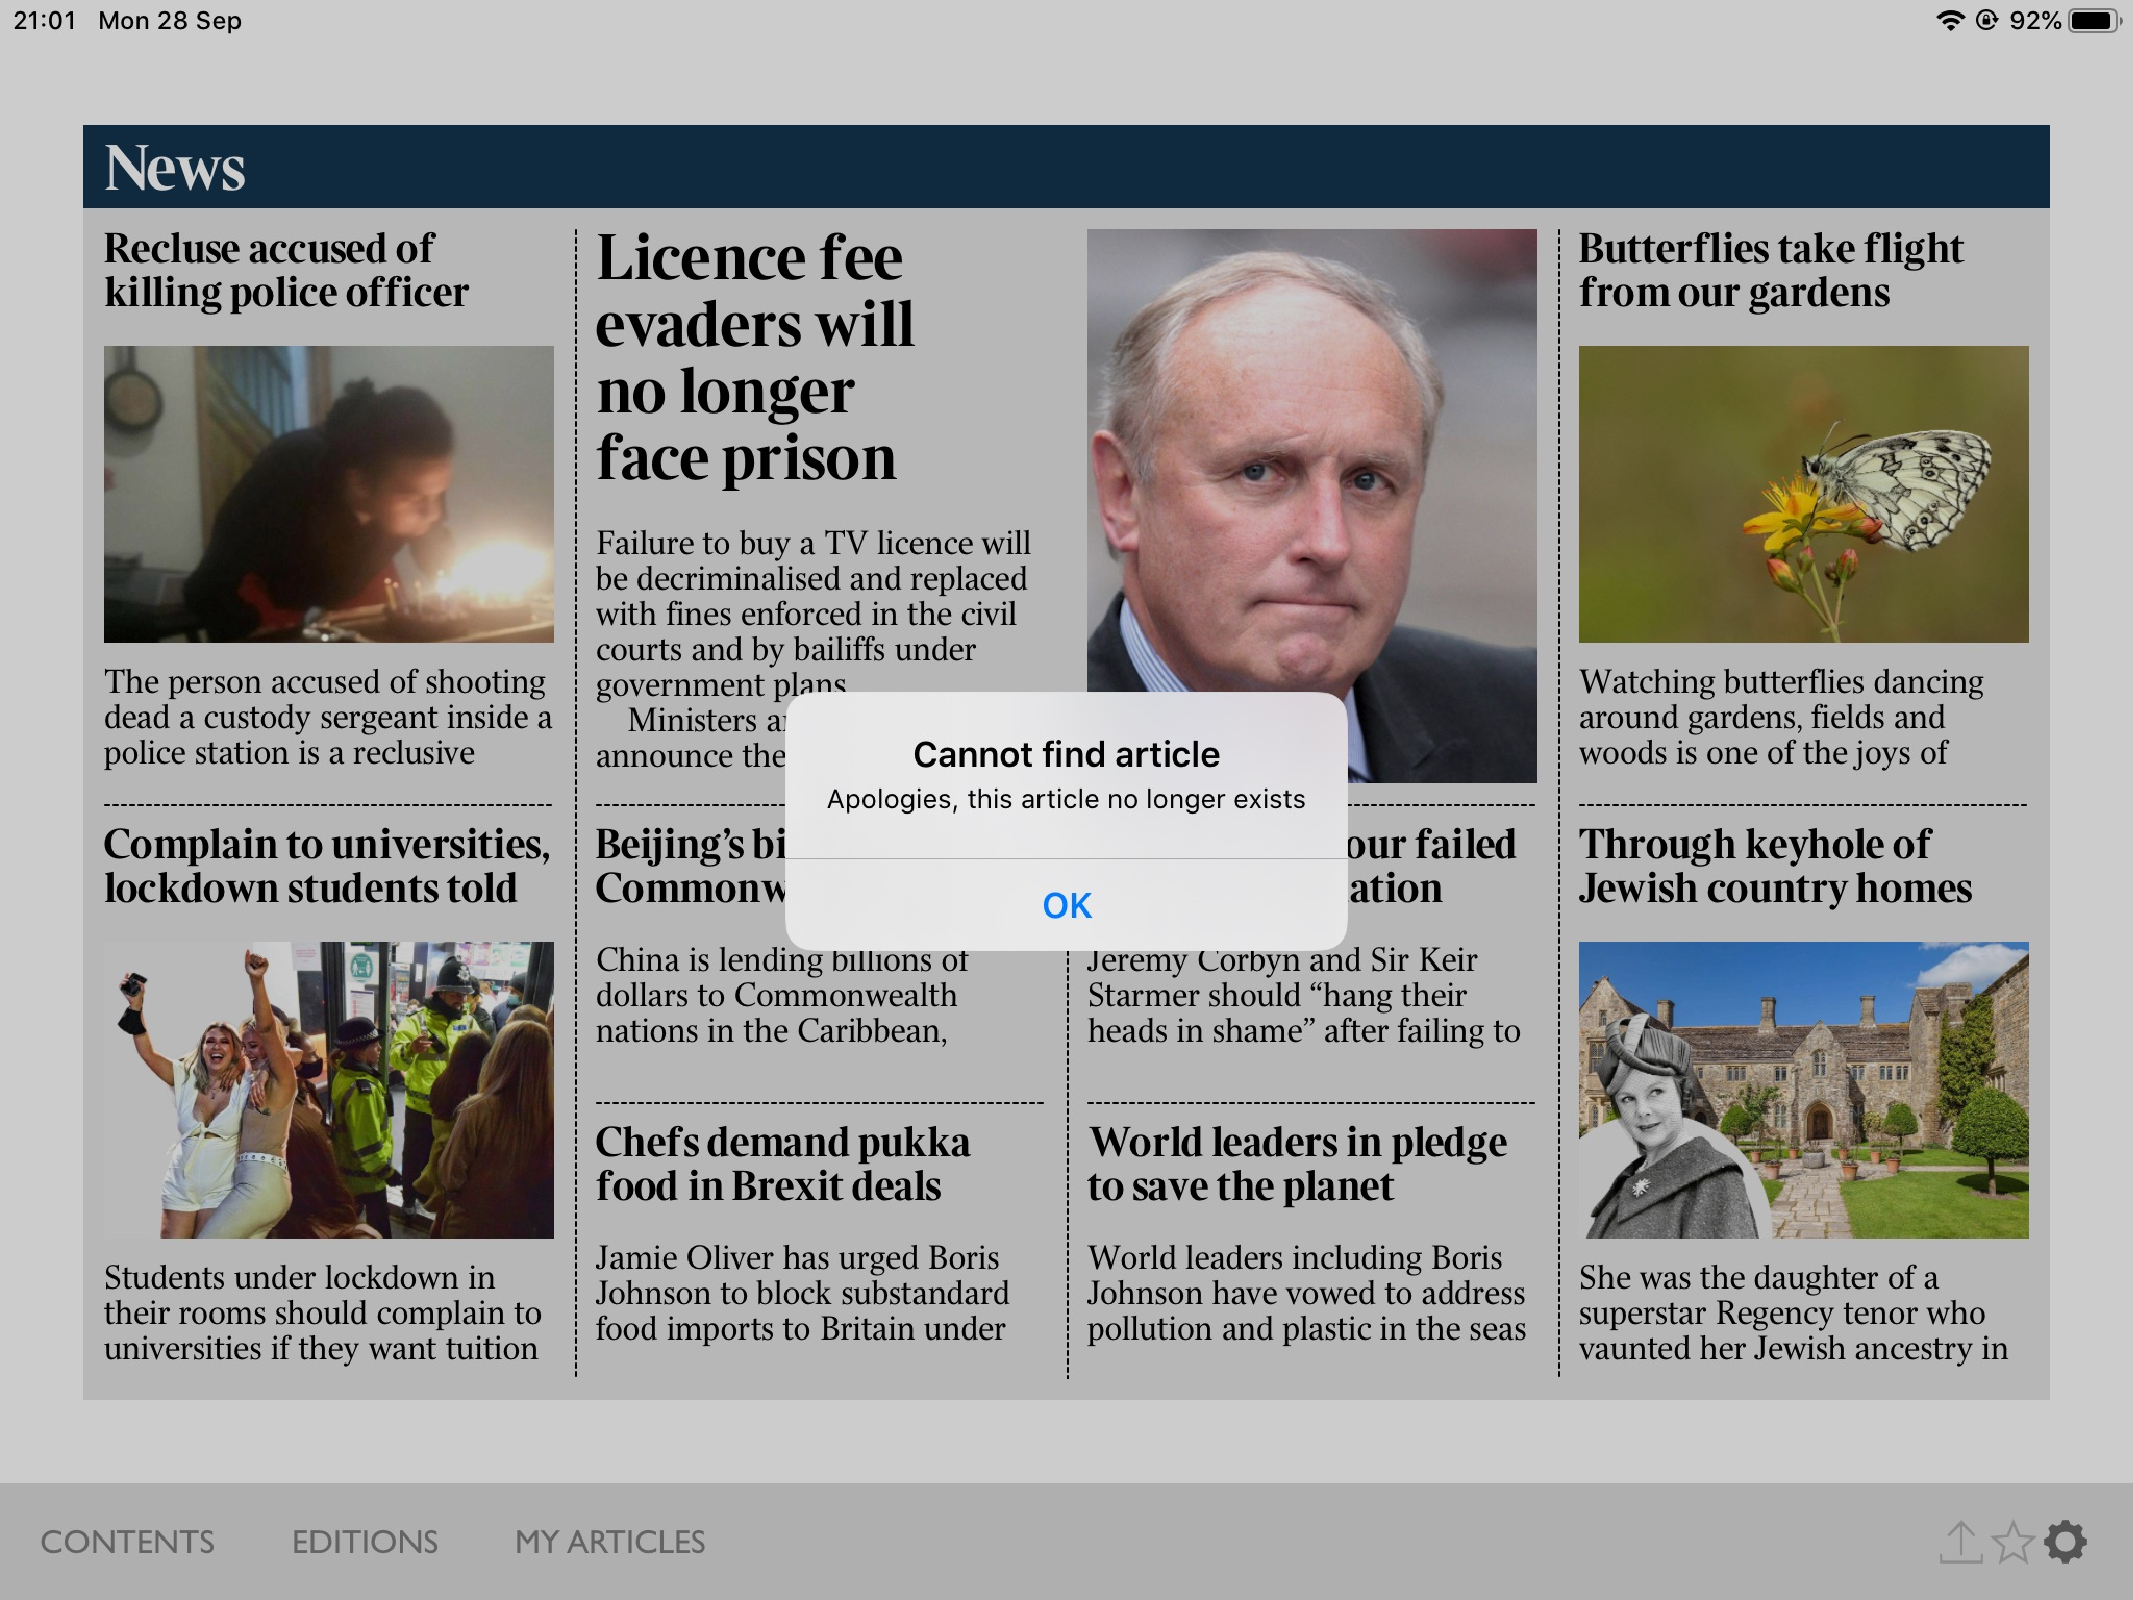
\includegraphics[width=13cm]{images/ios-screenshots/The-Times-iOS-Screenshot-2020-09-28.pdf}
    \caption{The Times iOS app: ``this article no longer exists" \nth{28} September 2020.}
    \label{fig:thetimes-ios-this-article-no-longer-exists}
\end{figure}
